\section{Results}
The entrainment ratios for all resonance profiles were averaged over all frequencies and all participants separately for each EEG channel. It was determined that there was a clear focal distribution of resonant power in the frontal cortex (Figure~\ref{fig:FocalDist}). Based on this focal distribution, resonance profiles for channel Fz were selected for all subsequent analyses.

Although the relationships between ASD traits (as measured by the BAPQ) and personality traits (as measured by the BFI-2S) were not related to the central hypotheses, it was essential to examine the degree of overlap between these traits, particularly in the context of interpreting how such overlap may influence differences in neural resonance (see Figure~\ref{fig:TikZmodel}).

\begin{figure}[ht!]
\centering
\begin{tikzpicture}[scale=.5,transform shape,auto,node distance=.9cm,
latent/.style={circle,draw,very thick,inner sep=0pt,minimum size=25mm,align=center},
manifest/.style={rectangle,draw,very thick,inner sep=0pt,minimum width=30mm,minimum height=10mm},
paths/.style={->, ultra thick, >=stealth'}]
\node [manifest] (SI) at (0,0) {Rigidity};
\node [manifest] (VO) [below=of SI] {Aloofness};
\node [manifest] (CO) [below=of VO] {Pragmaticism};
\node [latent] (g) [left=2.5cm of VO] {\emph{BAPQ Total}};
\node [latent] (Gc) [right=4.5cm of VO] {Conscientiousness\\ Negative Emotionality};
\foreach \all in {SI, VO, CO}
{
\draw [paths] (g.east) to node { } (\all.west);
}
\foreach \vc in {SI, VO, CO}
\draw [paths] (Gc.west) to node {} (\vc.east);
\end{tikzpicture}
\caption{\label{fig:TikZmodel} Significant Correlational Relationships between Personality and ASD Traits.}
\end{figure}

It was determined that there was a clear focal distribution of resonant power in the frontal cortex (Figure~\ref{fig:FocalDist}).

\begin{figure}[h!] 
\centering
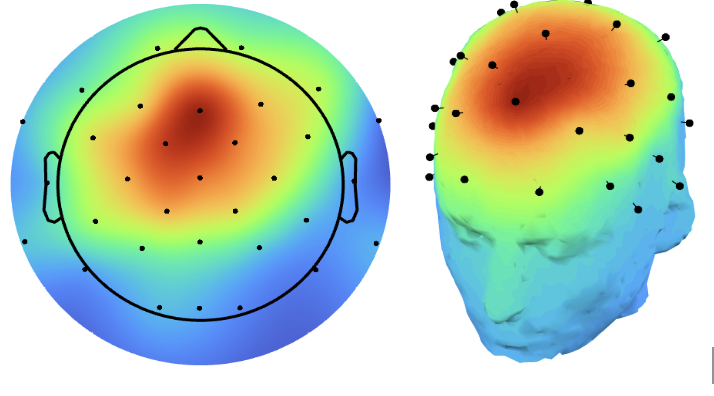
\includegraphics[width=0.3\textwidth]{Focal Dist.png}
\caption{\label{fig:FocalDist}EEG topographical maps of resonance peaks across all frequencies.}
\end{figure}

Descriptive statistics were computed for all key self-report measures, including the BAPQ subscales and the BFI-2S personality dimensions (see Table~\ref{tab:table1}).

\begin{table}[H]
\caption{Descriptive Statistics.}
\label{tab:table1}
 \begin{tabular}{l l c c c}
 \toprule
                          &              & \multicolumn{3}{c}{Week}\\
  \cmidrule{3-5}
                          &              & \textbf{One}    & \textbf{Two}    & \textbf{Three}\\
  \multirow{ 2}{*}{Group} & Experimental &     1008.435    &      986.76     &      859.1     \\
                          & Control      &     996.23      &      901.67     &      1002.23   \\
  \bottomrule
 \end{tabular}
\end{table}
